% -------------------------------------------------------
\section{Experimental Evaluation}
% -------------------------------------------------------

\subsection{Performance Metrics and Their Limitations}

The five methods represent fundamentally different analytic paradigms: unsupervised topic discovery, lexical counting, supervised classification, distributional drift, and dimensionality reduction. Each method requires a specific evaluation framework, yet none of the temporal analyses have an external ground truth for verification. Therefore, cross-method convergence is used as the primary standard of evidence. Findings that recur across methods with different representational assumptions carry more evidential weight than those from a single analysis. Table 1 summarises the metric choices and their principal limitations.
\begin{table}[H]
\centering
\caption{Performance metrics and key limitations by method}
\small
\setlength{\tabcolsep}{4pt}

\begin{tabularx}{\linewidth}{l >{\raggedright\arraybackslash}p{2.2cm} X}
\toprule
\textbf{Method} & \textbf{Metric(s)} & \textbf{Key Limitation} \\
\midrule
M1 Topic        & $C_v$ coherence score 
                & Rewards internal consistency; cannot penalise redundant topics or validate manual theory/application labelling \\
M2 Diffusion    & TF-IDF $\Delta$, Word2Vec cosine, SPECTER2 drift 
                & No absolute scale; SPECTER2 coverage constraint excludes most emergent terms by construction \\
M3 Framing      & Macro F1, Precision, Recall (5-fold CV) 
                & Top classifier features reflect broad topical vocabulary, not specifically limitation-framing language \\
M4 Dim. red.    & Pearson $r$, UMAP topology 
                & Centroid drift collapses within-year heterogeneity; TF-IDF PCA conflates temporal and subfield variance \\
M5 Lexical      & Raw term frequency (normalised by character count); TF-IDF weighted score per category per year
                & Vocabulary-bound: terms absent from the predefined list are invisible; likely understates the scale of the shift \\
\bottomrule
\end{tabularx}

\end{table}

M1-Topic modelling uses $C_v$ coherence, measuring how often the top words in a topic co-occur in short text segments. $C_v$ matches how people understand short documents and was chosen over held-out perplexity, which favors too many unclear topics and does not work well with short texts. $C_v$ finds the optimal number of topics but cannot evaluate manual labeling as theory- or application-focused; experts must judge that.

M2-Terminology diffusion combines three signals. Changes occur at the surface level through shifts in TF-IDF scores, at the word-meaning level via Word2Vec distances between aligned time periods, and at the overall topic level via SPECTER2 embedding changes. No single measure captures all three aspects. All scores are normalised to [0,1] across tracked terms; a threshold of (0.5, 0.5) on both axes produces the four-quadrant typology. SPECTER2 (allenai/specter2 via HuggingFace) was selected over general-purpose sentence encoders because its contrastive pretraining on citation pairs directly mirrors the semantic structure of a research abstract corpus.

M3-Limitation framing reports uses macro F1 as the main measure and five-fold stratified cross-validation. Macro averaging matters because the two periods, 2010–2013 and 2018–2020, have very different numbers of abstracts. Accuracy alone would mislead with overly positive results. Precision and recall are reported separately to show types of classification errors.

M4-Dimensionality uses the Pearson correlation between TF-IDF and Sentence-BERT year-to-year centroid distance series to measure consistency between representations. Distances are calculated in full-dimensional space: 50 components for TF-IDF after PCA, and 384 dimensions for SBERT. The 2D TF-IDF projection retains only about 1.6\% of total variance, so 2D centroid distances are unreliable. PCA and UMAP are both used for visualization; however, UMAP is only for visual purposes and does not provide numerical results.

M5-Lexical analysis compares raw term frequency (keyword count normalised by total characters per year) and mean TF-IDF score per keyword category. Comparing two scoring schemes is itself part of the experimental design: agreement in direction and timing strengthens the finding, while disagreement would flag a methodological artefact. The fundamental limitation is that the predefined keyword sets cannot capture newer application-oriented vocabulary, such as fine-tuning or zero-shot, almost certainly understating the true scale of the observed shift.

\subsection{Experimental Setup}
\paragraph{Corpus and temporal coverage.}
Temporal analyses use the same period structure described in Section~\ref{sec:methodology}: M5 and M3 operate on the full available range of 1990--2025 to capture the longest possible trajectory of lexical and limitation-framing change. M1, M2, and M4 operate from 2000 to 2021, where abstract volume is sufficient to support period-level topic models and embedding geometries. Corpus growth is severely skewed, and this is addressed differently across methods. M2 applies reliability weights of 0.27 and 0.49 to the two earliest periods to prevent sparse early corpora from distorting TF-IDF averages and Word2Vec training. M3 uses stratified folds to account for class imbalance. M4 and M5 compute per-year statistics without rebalancing, since the publication growth trajectory is itself a substantive empirical finding rather than a confound to be removed.
\paragraph{Preprocessing.}
A shared preprocessing pipeline was applied. All methods used the same preprocessing steps described in Section~\ref{sec:methodology}, including changing text to lowercase, breaking text into words, removing common words, and using WordNet to reduce words to their base forms based on their part of speech. However, for SentenceBERT and SPECTER2, the original abstracts, without base-form changes, were retained to preserve sentence structure and meaning. 
The temporal analyses (M1, M2, M4, M5): temporal ordering is the analytical design, not a holdout partition. M3 is the only exception. It uses a deliberately disjoint comparison of 2010–2013 versus 2018–2020, skipping the 2014–2017 transitional years to suppress noise during the period of change and sharpen the pre/post-neural-turn contrast. Five-fold stratified cross-validation is applied within this split.

\paragraph{Method-specific setup.}
For M1, the number of topics k was tested with values $\{6, 8, 10, 12\}$ for both LDA (Gensim) and NMF (scikit-learn). The setting that gave the best $C_v$ score was chosen: $k = 10$ for both models. LDA used simple word counts; NMF used TF-IDF features. Topics were labeled by hand, based on the top 10 words for each topic and classifying them as theory-focused, application-focused, or method-focused.

For M2, candidate terms were mined by computing per-period TF-IDF on a concatenated period corpus (\texttt{sublinear\_tf=True}) and retaining the top-60 rising terms. Approximately 37\% were removed as subsumed $n$-grams, yielding approximately 48 candidates. Before Word2Vec training, 174 multi-word compounds (e.g., \texttt{word\_embeddings}, \texttt{pre\_training}) were merged into underscored tokens to prevent spurious decomposition. Word2Vec skip-gram models (\texttt{vector\_size=300}, \texttt{window=12}, \texttt{min\_count=2}, \texttt{negative=10}, \texttt{epochs=30}, \texttt{seed=42}) were trained per temporal period; \texttt{window=12} was chosen over the default 5 to capture longer-range scientific context, given the longer mean sentence length of abstracts. Cross-period alignment used Procrustes orthogonal transformation (\texttt{scipy.linalg.orthogonal\_procrustes}) on 1,436 shared anchor terms. For SPECTER2, encoding used raw non-lemmatised abstracts (batch size 64, L2-normalised outputs via \texttt{\seqsplit{SentenceTransformer("allenai/specter2\_base")}}), with lemmatisation applied only at the term-detection layer. Bootstrap aggregation resampled abstracts $B = 100$ times per (term, period) cell; cells with fewer than 5 abstracts were excluded, leaving 30 of 48 candidate terms with full SPECTER2 coverage.

\subsection{Results}
\subsubsection{Theory-to-Application Shift}
M5, M1, and M4 converge independently on approximately 2014–2016 as the primary inflection point. Under M5, application-oriented keyword prevalence overtakes theory-oriented prevalence in 2014 under raw frequency scoring and in 2015 under TF-IDF, with both measures showing a sustained upward trend through 2025 and no reversal. The one-year difference between scoring schemes falls within the expected noise of TF-IDF's corpus-relative scaling. The directional finding is stable across both vocabulary sizes tested: a focused 9-term set and a broader 29-term set agree on direction, though the larger set introduced noise from semantically ambiguous terms such as model and method that appear with nearly equal frequency in theoretical and applied contexts, supporting the choice of the narrower vocabulary.
Topic modelling (M1) corroborates this independently and without predefined vocabulary. NMF with 10 topics achieved the highest coherence across all configurations ($C_v = 0.55$, Table 3). Topics dominated by algorithm, optimisation, convergence, statistical, estimation, and inference were labelled theory-oriented; topics dominated by dataset, prediction, healthcare, translation, recommendation, and platform were labelled application-oriented. Tracking proportions over time shows an uninterrupted rise in application-oriented topic share from the early 2000s through 2021. Critically, both LDA and NMF recover this trend despite their different mathematical assumptions. LDA through probabilistic topic assignment, NMF through non-negative matrix factorisation of TF-IDF features, which constitutes evidence that the signal reflects genuine structure in the data rather than the inductive bias of either model.

\begin{table}[H]
\centering
\caption{Topic coherence scores by model and configuration}
\small

\begin{tabular}{llcc}
\toprule
\textbf{Model} & \textbf{Representation} & \textbf{Topics} & \textbf{$C_v$} \\
\midrule
LDA & BoW     & 6  & 0.43 \\
LDA & BoW     & 8  & 0.46 \\
LDA & BoW     & 10 & 0.48 \\
NMF & TF-IDF  & 6  & 0.49 \\
NMF & TF-IDF  & 8  & 0.52 \\
NMF & TF-IDF  & 10 & \textbf{0.55} \\
\bottomrule
\end{tabular}
\end{table}
Dimensionality reduction (M4) provides the strongest cross-representation corroboration. The Pearson correlation between TF-IDF and the Sentence-BERT year-on-year centroid distance series is $r = 0.863$, indicating that two fundamentally different representations independently track the same temporal rhythm of change. Both representations place 2014–2016 as the highest-movement window (Table 3). The most counterintuitive result is that 2017 ranks last in both representations despite being the year of the Transformer paper. This is mechanistically principled: the 2017 corpus reflects work already in progress before the Transformer architecture existed. Corpus-based analysis records the diffusion of ideas at scale, not their point of origin. The paradigm shift registers approximately 12 to 24 months after publication, when citing papers adopt the vocabulary at scale.
\begin{table}[H]
\centering
\caption{Year-on-year centroid distance rankings (selected years)}
\small
\begin{tabularx}{\linewidth}{l c c X}
\toprule
\textbf{Year} & \textbf{TF-IDF} & \textbf{SBERT} & \textbf{Interpretation} \\
\midrule
2014 & 0.655 (5th)          & 0.890 (3rd) & Neural transition begins, SBERT starts showing stronger structure sensitivity \\
2015 & 0.754 (4th)  & 0.935 (2nd) & Peak neural adoption and embedding stabilization effects \\
2016 & 0.959 (2nd)  & 0.831 (4th)         & Highest TF-IDF centroid shift, strong lexical drift observed \\
2017 & Lowest       & Lowest      & Transitional stability period, reduced semantic displacement \\
2018 & High (3rd)   & Moderate (5th) & BERT-era emergence with secondary structural realignment \\
\bottomrule
\end{tabularx}

\end{table}

\begin{figure}[H]
\centering
\fbox{\parbox{0.9\columnwidth}{\centering\small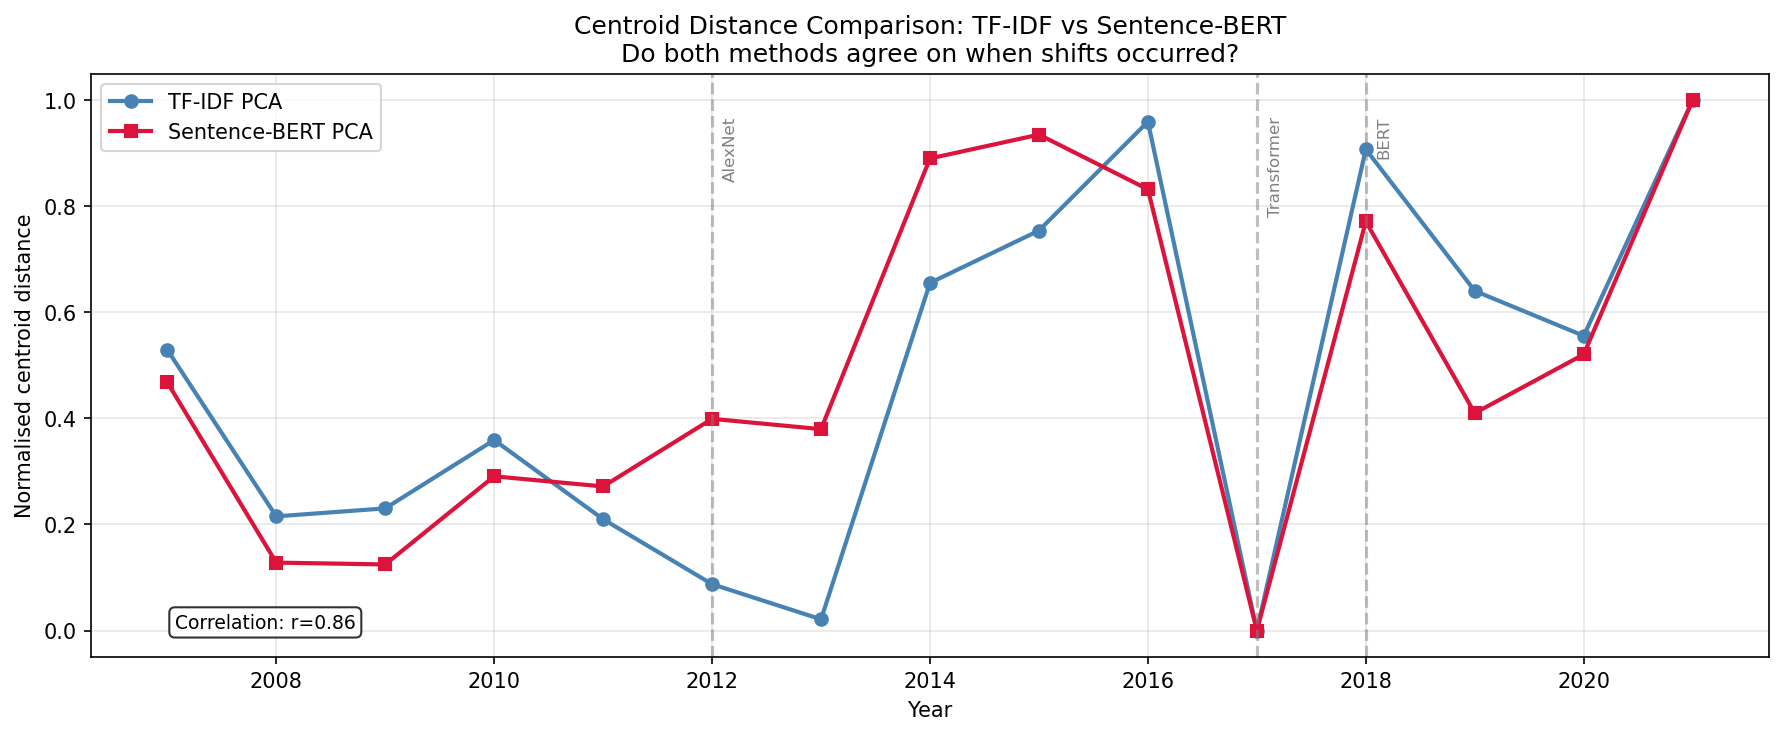
\includegraphics[width=0.9\columnwidth]{figures/pca_figures/fig3.png}}}
\caption{Year-on-year centroid distance comparison, TF-IDF vs.\ SBERT}

\end{figure}

\setcounter{figure}{4}

While the two representations agree on the timing of major shifts, they differ in sensitivity. Sentence-BERT assigns higher relative movement to earlier years within the transition (e.g., 2014–2015), whereas TF-IDF peaks later (2016), consistent with a lag in vocabulary adoption relative to underlying conceptual change. This supports H4, indicating that semantic and lexical signals are not perfectly synchronous but remain directionally aligned.

\textbf{Extended Embedding Structure Analysis}

Post-hoc analysis of Sentence-BERT embeddings is consistent with TF-IDF PCA and confirming that the largest sources of variance arise from disciplinary differences rather than temporal change. Nearest-neighbour analysis (using the BERT paper as a probe) validates semantic coherence and reveals a diffusion effect, where follow-on work (2019–2020) clusters more closely than contemporaneous papers, indicating that embedding space reflects intellectual influence and reinforcing the finding that corpus-based methods capture the spread of ideas rather than their origin. K-means clustering (k = 8) further supports the interpretation that the field has expanded rather than replaced its structure, with declining symbolic AI, stable core task clusters, and emergent neural systems, and safety-related research coexisting over time. Crucially, extending PCA beyond the standard 2D projection shows that temporally coherent signals emerge only in higher-order components, with PC4 exhibiting a strong monotonic trend (Kendall's $\tau = +0.667$, $p < 0.001$)  corresponding to the rise of socially-aware AI research (e.g., fairness, interpretability, ethics), a signal entirely invisible in 2D due to its orthogonality to dominant variance. This demonstrates that meaningful temporal dynamics exist in directions not aligned with the largest variance components, and that low-dimensional projections alone can obscure key patterns of field evolution.

\begin{figure}[H]
\centering
\fbox{\parbox{0.9\columnwidth}{\centering\small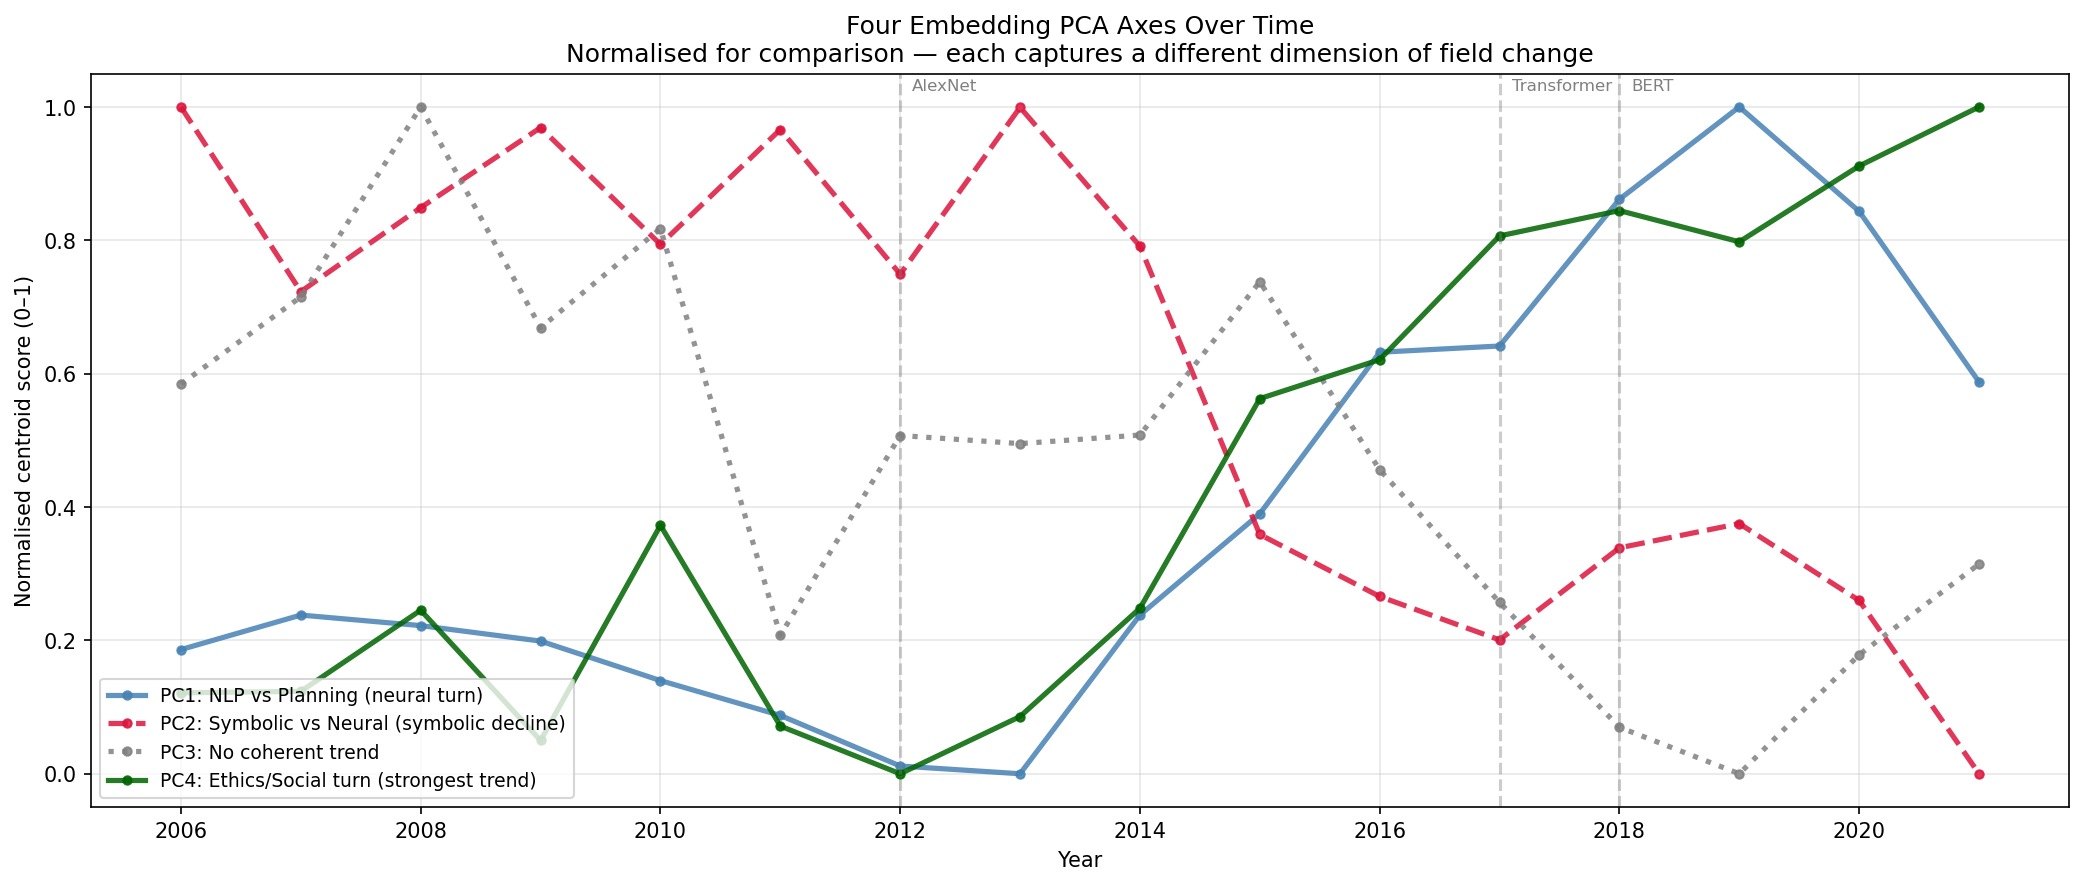
\includegraphics[width=0.9\columnwidth]{figures/pca_figures/fig4.png}}}
\caption{Fig.\ 4: Embedding PCA components over time}
\end{figure}

\subsubsection{Limitation Framing}

The four-category lexical analysis reveals distinct temporal trajectories across framing types. Hedging language (could, may) was consistently present across all periods, suggesting it is a stable feature of academic register rather than a response to any specific development. Capability language (limited, cannot) was the most common category in early periods but declined steadily from approximately 28\% in 1990 to 22\% by 2020–2021. Failure language (fail, degrade) began low at around 6\% and grew to become the second most prevalent category by 2020–2021 at approximately 24\%, reflecting the increasing emphasis on empirical benchmarking and performance comparison. Ethics language (bias, fairness) was near-absent before 2015 and rose to $\approx$ 13\% of abstracts by 2020–2021, a trajectory that directly parallels the large-scale deployment of AI systems in socially consequential contexts.
\setcounter{figure}{4}
\begin{figure}[H]
\centering
\fbox{\parbox{0.9\columnwidth}{\centering\small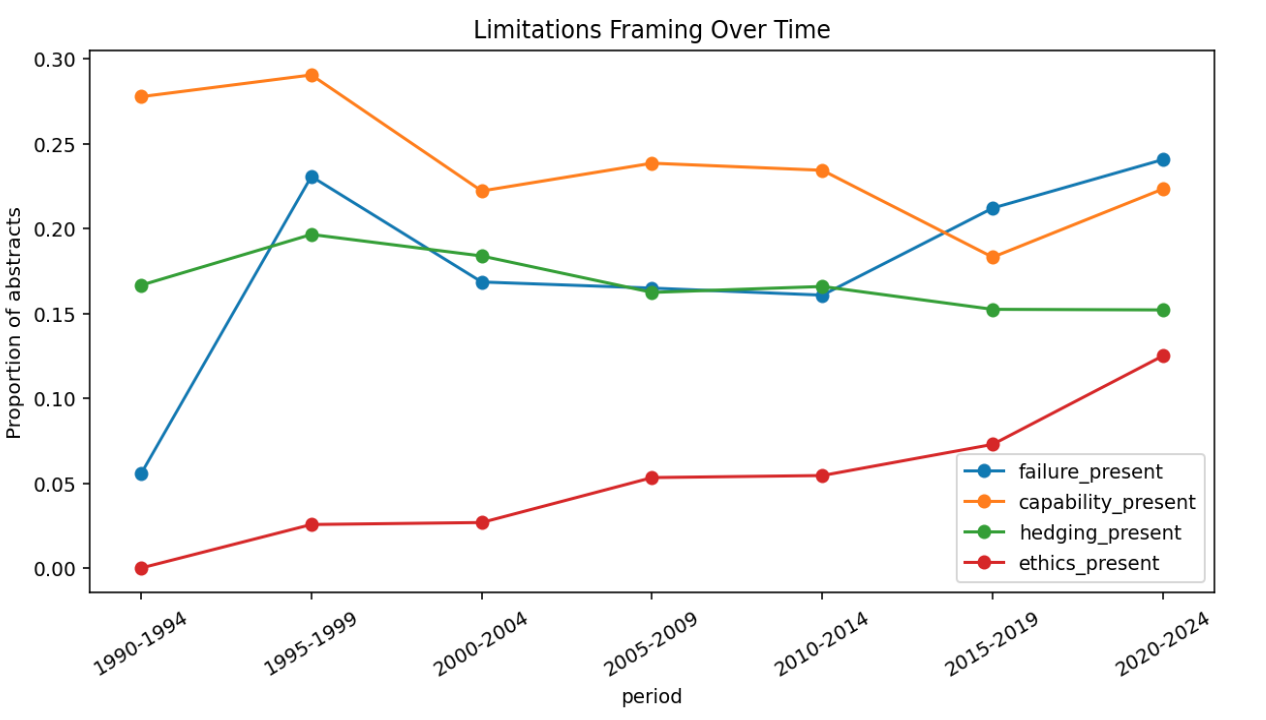
\includegraphics[width=0.9\columnwidth]{figures/limitation_framing/limitation1.png}}}
\caption{Proportion of abstracts containing each limitation framing category across time. Ethics language shows the sharpest rise post-2015.}
\end{figure}

Notably, method-introducing and non-method abstracts show near-identical rates of limitation language (51.4\% vs. 51.1\%), indicating that limitation framing has become a normalised feature of academic writing across research types rather than a marker of methodological modesty in technically focused papers.
The binary classifier achieved a mean cross-validation accuracy of 85.8\% with macro F1 scores of 0.71 for the early period (2010–2013) and 0.92 for the late period (2018–2020).


\begin{table}[H]
\centering
\caption{Classification performance (5-fold CV)}
\small

\begin{tabularx}{\linewidth}{l c X}
\toprule
\textbf{Period} & \textbf{F1} & \textbf{Observation} \\
\midrule
Early (2010--13) & 0.71 & Minority class; higher variance; more diverse vocabulary \\
Late (2018--20)  & 0.92 & The majority class is dominated by consistent neural-era vocabulary \\
Mean CV Acc.     & 85.8\% & Macro-averaged to correct for class imbalance \\
\bottomrule
\end{tabularx}

\end{table}
The F1 gap reflects the class imbalance between periods and the greater lexical consistency of late-period abstracts, which are dominated by a relatively stable neural-era vocabulary. The high overall accuracy confirms that the two periods are robustly distinguishable from abstract text alone.

\begin{figure}[H]
\centering
\fbox{\parbox{0.9\columnwidth}
{\centering\small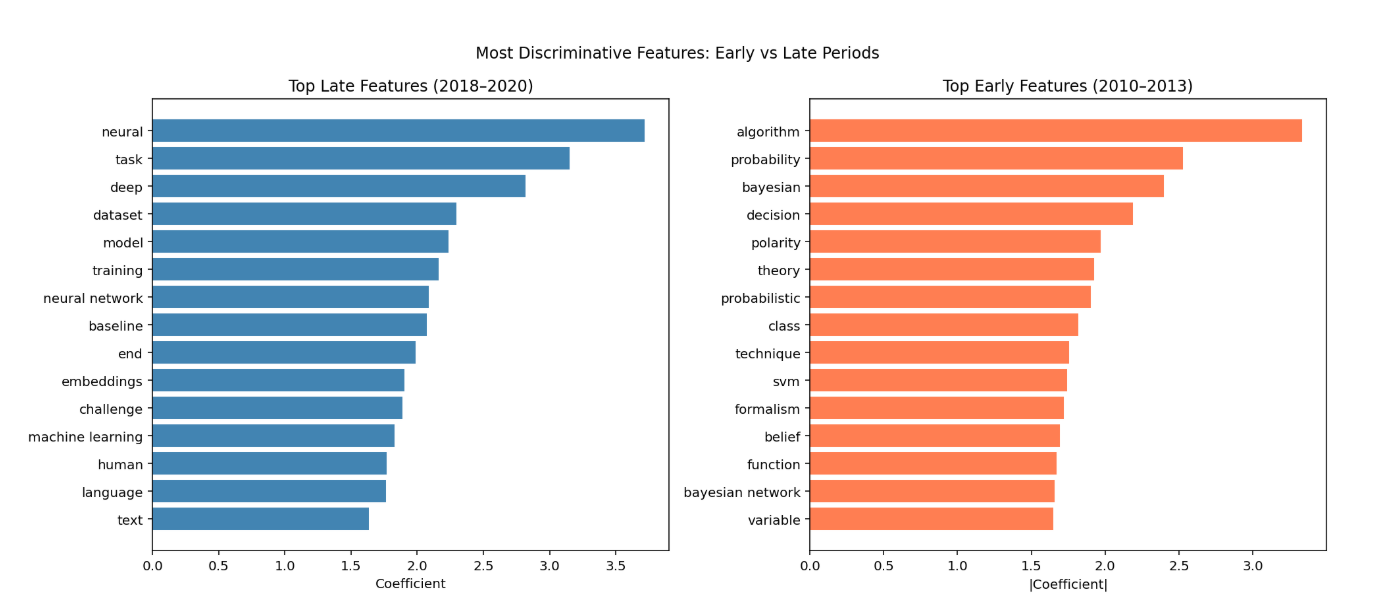
\includegraphics[width=0.9\columnwidth]{figures/limitation_framing/limitation2.png}}}
\caption{Top discriminative features for the early (2010--13) and late (2018--20) periods. Features reflect broad topical change rather than limitation-specific language.}
\end{figure}

Cosine distance between five-year period centroids reveals two statistically distinct transitions: 1990–1994 to 1995–1999 (distance = 0.349) and 2010–2014 to 2015–2019 (distance = 0.303). All other consecutive period pairs show substantially smaller distances (0.09–0.19), confirming that the limitation discourse evolves through discrete phase transitions rather than gradual continuous drift. PCA trajectories show stable semantic positioning from 1990 to 2014, a sharp shift from 2015 to 2019, and gradual stabilisation thereafter (distance = 0.090).

\subsubsection{Terminology Diffusion}

The four-quadrant typology classifies 36 tracked terms across two axes: normalised TF-IDF rise and mean W2V + SPECTER2 drift, thresholded at (0.5, 0.5).

\begin{figure}[H]
\centering
\includegraphics[width=\columnwidth]{figures/terminology_diffusion_figures/Fig7.png}
\caption{Four-quadrant diffusion typology.}
\label{fig:terminology_diff}
\end{figure}

The largest category is Semantic Shift Only ($n = 13$), followed by Stable/Peripheral ($n = 16$), Diffused ($n = 6$), and a singleton Actively Diffusing quadrant occupied by \textit{pre-training}. This distribution challenges frequency-centric accounts of terminology adoption: the dominant diffusion pathway in this corpus is quiet conceptual repositioning that is entirely invisible to frequency-only analysis.

\begin{figure}[H]
\centering
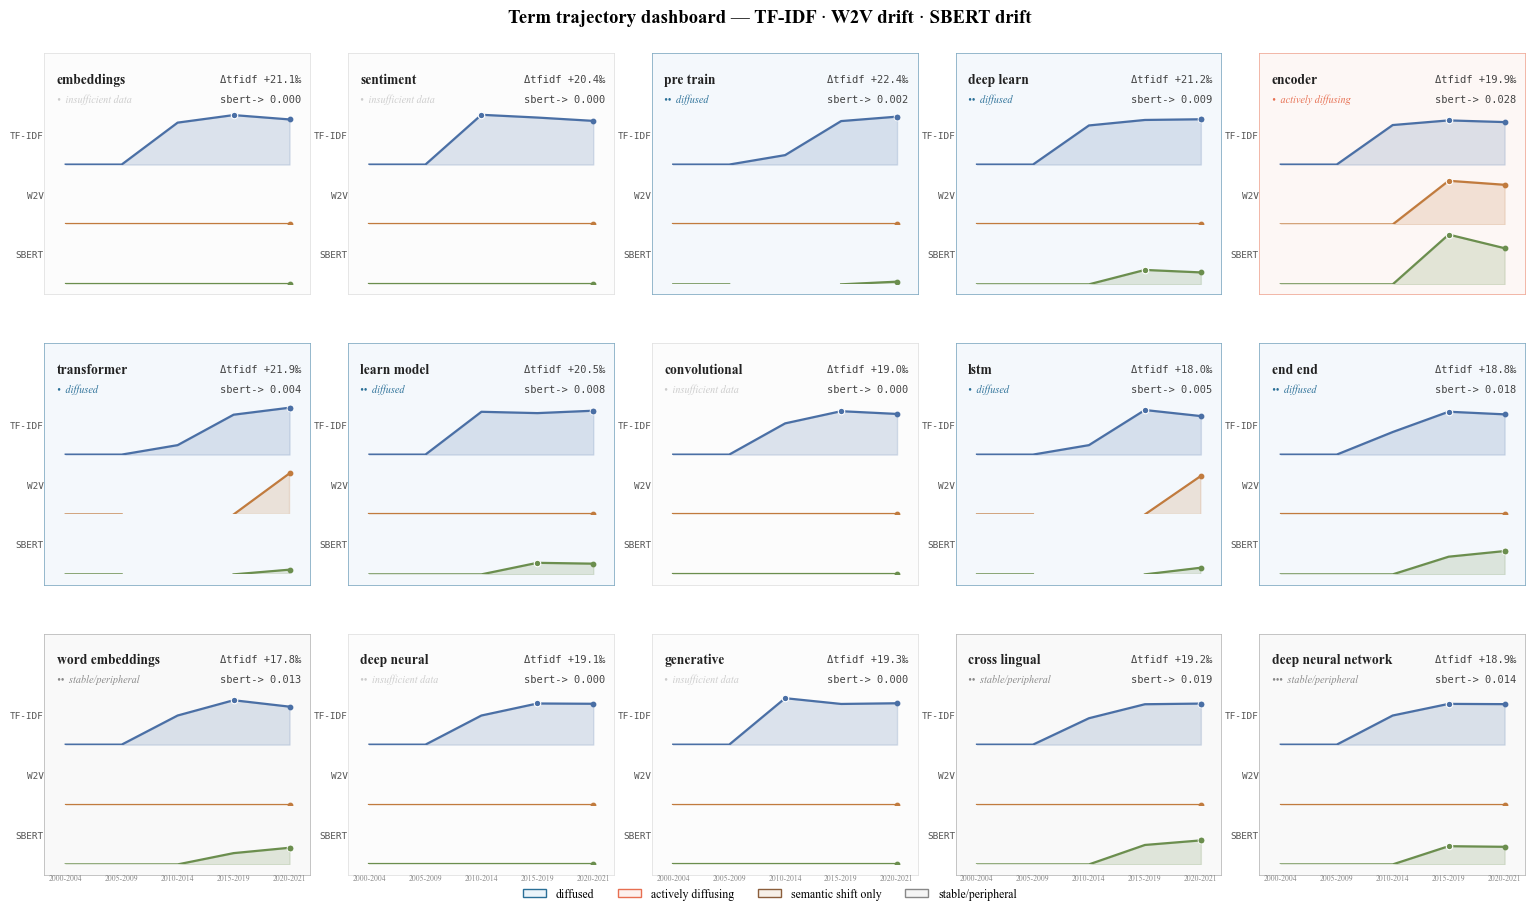
\includegraphics[width=\columnwidth]{figures/terminology_diffusion_figures/Fig8.png}
\caption{Per-term trajectory cards showing TF-IDF, W2V, and SPECTER2 signals across five periods. Card colour encodes the diffusion quadrant.}
\label{fig:terminology_diff}
\end{figure}

\textit{Encoder} case provides the clearest convergent evidence across all three signals, achieving the highest consensus score (0.63) and highest SPECTER2 drift (0.0424). Visual inspection of the neighbour replacement ribbons confirms near-total neighbourhood replacement across periods Jaccard $\approx$ 0.001, demonstrating that the term's distributional context changed completely between the earliest and latest periods.

\begin{figure}[H]
\centering
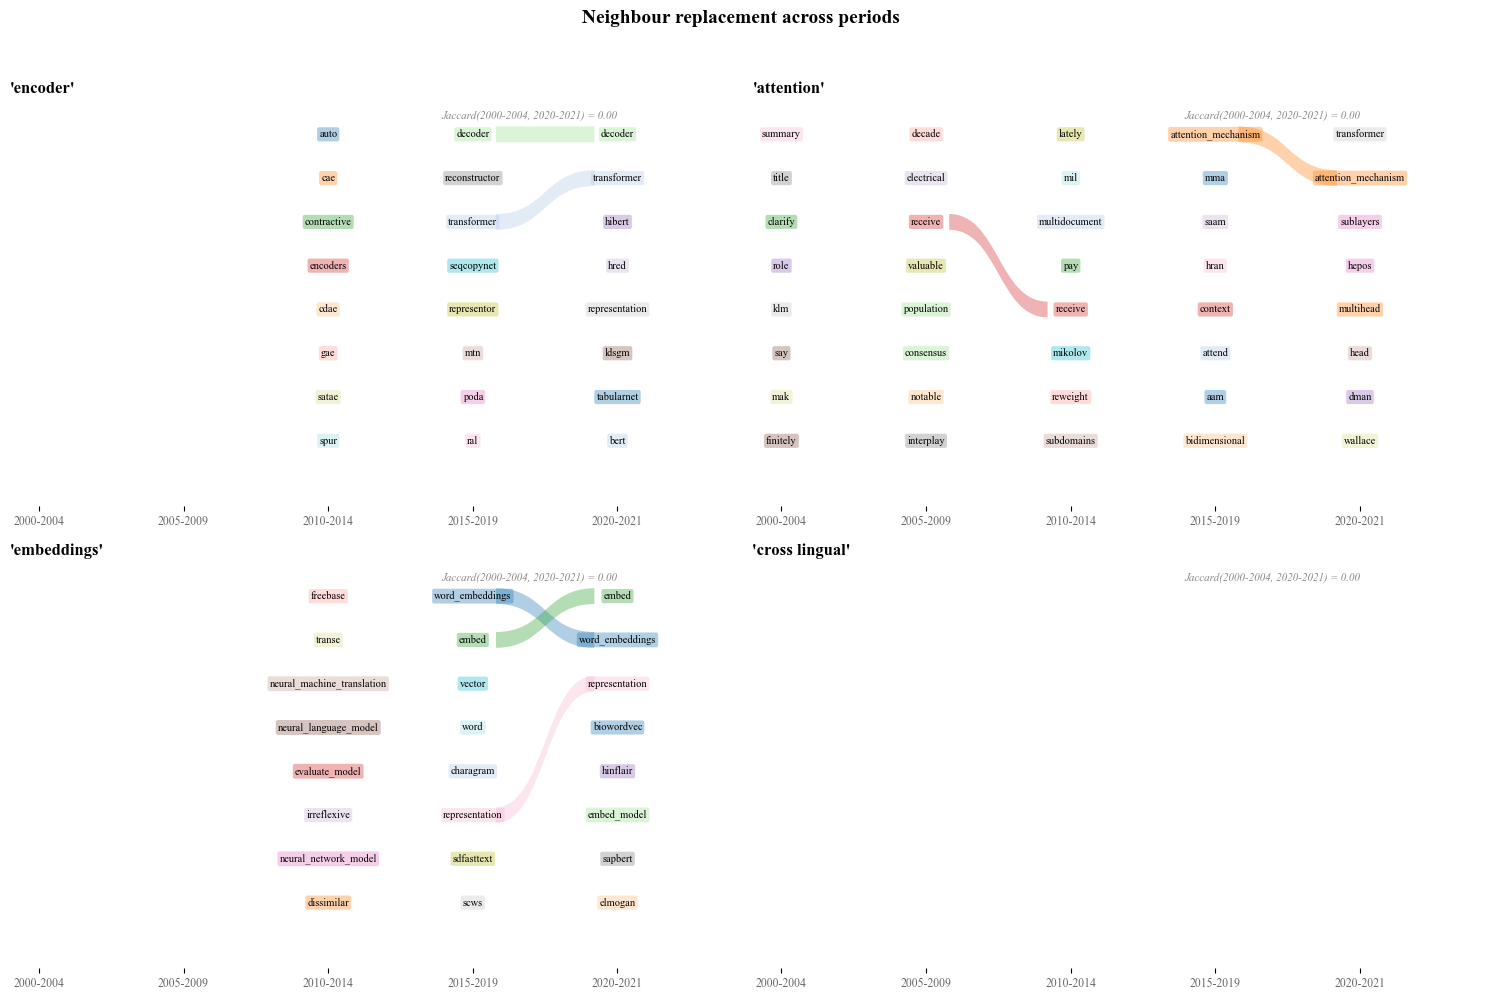
\includegraphics[width=\columnwidth]{figures/terminology_diffusion_figures/Fig9.png}
\caption{Neighbour replacement ribbons across periods. \textit{Encoder} shows near-total replacement.}
\label{fig:terminology_diff}
\end{figure}

The counterexample is pre-training: highest TF-IDF rise ($\approx$0.84) but near-zero SPECTER2 drift (0.0021). This identifies it as a discourse template replication event. The BERT fine-tuning argumentative structure was established in a small number of pioneering papers and reproduced at scale with minimal variation, producing a terminological monoculture rather than conceptual diffusion.

\subsection{Error Analysis}

\textbf{Topic Modeling Ambiguity (M1)}

Manual labeling involves unavoidable personal judgment for mixed topics. A topic focused on neural architecture and deep layers was labeled as methodological but could reasonably fit under either theory or application, since many NLP abstracts report both architectural innovation and practical task use. This is a basic limitation of bag-of-words methods: themes that appear together cannot be separated within a single abstract, so topics that span both sides get a single, approximate label. Theory/application proportion curves should be seen as general trends rather than exact measurements. LDA is more affected by this than NMF, as its lower coherence scores indicate less clear topic boundaries and less consistent labeling across runs.

\textbf{Diffusion Coverage Bias (M2)}

The SPECTER2 rule requires at least 5 abstracts per term-period group excludes new terms such as transformer, downstream task, low resource, and prompt, which did not appear before 2010–14 and thus lack an early reference point for measuring change. This causes a consistent underestimation of the most important terms. The uneven coverage stems from how the metric is designed and cannot be attributed to random error. The Procrustes alignment adds to this problem: only 1,436 of 20,631 combined vocabulary terms (6.9\%) appear in all time periods. For terms that change a lot and are surrounded by time-specific words missing from the reference set, alignment errors can still happen unless the size of the reference vocabulary is tested for sensitivity.

\textbf{Classification Errors (M3)}

The confusion matrix shows a clear one-sided imbalance: 108 late-period abstracts were mislabeled as early, while only 35 early abstracts were mislabeled as late. This imbalance is intentional. The misclassified late abstracts consistently use older vocabulary, such as Bayesian inference, causal modeling, and formal semantics, even in 2018–2020. The classifier learned the main late-period language but misses the smaller group of late papers that avoid neural-era terms, creating a distinct subgroup rather than random errors. Early abstracts are rarely mislabeled as late because their older vocabulary is very distinctive and almost never appears in later work.

A bigger problem appears when looking at the top distinguishing features. The most predictive words are algorithm, Bayesian, probability (early), and neural, deep embeddings (late). These are broad topics, not specific words for limitations. Only one of the top classifier features matches the manually created limitation keyword lists. So, the classifier is tracking the overall vocabulary change in the subfield, not changes in how limitations are described, mixing a related factor with the main signal. This limits how well it can directly show language evolution, even though its overall accuracy is good.

\textbf{PCA Failure (M4)}

Using PCA on TF-IDF vectors reveals a basic limitation. The main components reflect the vocabulary of different subfields instead of changes over time. The first component is influenced by NLP-related words like language, word, translation, and sentence, and separates cs.CL from cs.LG and cs.AI. So, the biggest source of variation shows the mix of disciplines rather than evolution. There is also a significant loss of information: 2D PCA captures only 1.6\% of the total variation, and even 50 components capture only about 14\%. This reduces the reliability of centroid-based analysis.

Sentence-BERT embeddings show a similar problem. The main components capture differences between disciplines - such as NLP versus broader AI and symbolic versus connectionist approaches not changes over time. Since embedding dimensions cannot be directly understood, they have to be inferred qualitatively. Time-related patterns appear in less important components, confirming that time is not a main source of variation. Variation within each year decreases over time, even as average positions shift, showing the field moves along a common path rather than splitting into separate directions.

\subsection{Discussion}

\textbf{Cross-Method Convergence}

Importantly, it is not the results of any single experiment that matter, but that all five methods point to 2014-2016 as the key turning point. Word counts (M5) change around 2014-2015; application-focused topic counts (M1) keep rising during this time; TF-IDF and Sentence-BERT centroid distances (M4, $r = 0.863$) reach their highest points independently here; Word2Vec (M2) drift curves show a clear shift from 2010-2014 to 2015-2019 for tracked terms. Despite their different ways of working and scale, their agreement strongly shows that this turning point is a real feature of the data, directly supporting H4.

\textbf{Expansion, Not Replacement}

This is more about growth than replacement. UMAPs show all time periods mixed together in the meaning space. Theory-focused topics make up a smaller part of the field, but still exist; most tracked terms just moved position. At the same time, variation within years decreases, showing that the field is uniting around methods and evaluation practices, adding new application-focused practices while maintaining a core theoretical base. Methods that look for replacement (like losing keywords) will overestimate how much the field is breaking apart.

\textbf{Hypothesis Results}

H1 verified: the NMF recovered the paradigm shift and hybrid topics that were missed by the keywords. H2 confirmed on the encoder case, but SPECTER2's coverage constraint blocks testing the most emergent terms. H3 partially confirmed: centroid measures captured the 2017 lag, but classification captured between-period separability but conflated topical and framing effects. H4 is very strongly supported by five-fold convergence on 2014-2016. 

\textbf{Comparative Strengths and Recommendations}

Manual vocabulary analysis (M5) is easy to understand but depends on specific words, so it gives a minimum estimate of the shift. Topic modeling (M1) removes the vocabulary limit, and agreement between LDA and NMF builds confidence, but the bag-of-words model mixes topics that appear together, and naming them is subjective. Dimensionality reduction (M4) is the best method for cross-checking results, but it should be checked to ensure changes are not due solely to shifts in subfields. Terminology diffusion (M2) is the most unique: the 13-term Semantic Shift Only group and the pre-training template replication result appear only in diffusion; the limited Procrustes anchoring of diffusion (6.9\% of the combined vocabulary) cannot rule out alignment errors for terms with large changes. Classification (M3) is the only method with a numeric measure of how well it generalizes, but it mixes topic words with language specific to limitations.

Three improvements would greatly help future work: expanding the collection beyond 2021 to clarify ongoing diffusion trends for cross-language and benchmark; replacing simple two-period classification with a sequence model to find when framing changed instead of just showing two separate periods; and repeating analyses on full paper texts to see if the almost identical amount of limitation language in different paper types (51.4\% vs. 51.1\%) means normalization or abstract-genre normalization.